\cleardoublepage
\chapter{Descripción informática}

Descripción del proyecto realizado. Después de unos párrafos introductorios el capítulo se divide en subcapítulos. (de 25 a 35 páginas)

\section{Requisitos}
\label{sec:requisitos}

Descripción detallada de las funcionalidades que tendría que implementar la aplicación (pues se asume que los requisitos se escriben antes de empezar el desarrollo). Pueden tener forma de historias de usuario o bien ser una lista de requisitos funcionales y no funcionales.

\section{Arquitectura y Análisis}
\label{sec:arquitectura-analisis}

Descripción de los aspectos de alto nivel de la aplicación. Diagramas de clases de análisis, diagramas de clases de diseño, etc. Se debe incluir la suficiente información para que el lector pueda entender la estructura de alto nivel del software desarrollado. Se pueden incluir diagramas de casos de uso si se considera útil.

\section{Diseño e Implementación}
\label{sec:diseno-implementacion}

Descripción de algún aspecto relevante de la implementación que quiera mencionarse. Por ejemplo se podría incluir alguno de los siguientes aspectos:
\begin{itemize}
  \item Algoritmo complejo que se haya tenido que desarrollar.
  \item Integración entre librerías problemática.
  \item Resolución de algún bug que haya sido especialmente problemático.
  \item Focalizar en alguna parte del desarrollo y describirla en más detalle.
\end{itemize}

En esta sección se pueden incluir fragmentos de código fuente. También se pueden incluir algunas métricas del proyecto (número de clases, líneas de código, etc.). También se puede incluir la evolución del repositorio de GitHub (gráfico de commits por día).

\section{Pruebas}
\label{sec:pruebas}

En esta sección se describen las pruebas automáticas que han sido implementadas para el proyecto. Sobre los tests, conviene indicar la cobertura del código. Si no se han implementado pruebas automáticas, deberían haberse implementado y describirse aquí o tener una buena justificación de por qué no se han implementado.


\section{Requisitos}
\label{sec:requisitos}

La aplicación \textbf{Pinche} nace con el objetivo de facilitar la organización de la compra doméstica mediante una herramienta móvil accesible, intuitiva y práctica. Para ello, se han definido una serie de requisitos funcionales que reflejan las necesidades del usuario final, así como requisitos no funcionales que garantizan la calidad del sistema.

\subsection{Requisitos funcionales}

Para definir los requisitos funcionales se ha seguido una metodolog\'ia personalizada que combina las fortalezas de las metodolog\'ias \textbf{Scrum}, \textbf{Kanban} y \textbf{Extreme Programming (XP)}. Se ha seguido la estructura iterativa de Scrum, utilizando tableros Kanban para visualizar el flujo de tareas y adoptando buenas pr\'acticas como pruebas continuas e integraci\'on frecuente propias de XP.

La organizaci\'on del desarrollo ha comenzado con la definici\'on de \textbf{historias de usuario}, expresadas en el formato: ``Como [tipo de usuario], quiero [funcionalidad] para [beneficio]''. Estas historias fueron elaboradas y refinadas por el equipo de desarrollo en conjunto con el Product Owner, y se han estimado mediante la t\'ecnica de \textbf{Story Points} basada en la sucesi\'on de Fibonacci (1, 2, 3, 5, 8, 13).

Las historias se han agrupado en \textbf{\'epicas}, agrupaciones l\'ogicas que organizan funcionalidades principales: \textit{Cuenta de usuario}, \textit{Lista de la compra}, \textit{Recetas} e \textit{Invitados}.


La épica \textit{Cuenta de usuario} agrupa un total de seis historias de usuario con sus respectivas tareas que tienen como objetivo toda la gestión dentro de la aplicación de la cuenta del usuario. Las historias de usuario serian:

\begin{enumerate}
  \item Como usuario, necesito registrarme en la aplicación con la finalidad de poder utilizarla. Estimación: 2 puntos de historia.
  \item Como usuario, necesito iniciar sesión en la aplicación con la finalidad de acceder a mi cuenta de usuario y mis datos. Estimación: 1 punto de historia.
  \item Como usuario, necesito cerrar sesión en la aplicación con la finalidad de no dejar mi cuenta activa en un dispositivo. Estimación: 1 punto de historia.
  \item Como usuario, quiero recuperar mi contraseña de mi cuenta de usuario de la aplicación con la finalidad de poder acceder a mi cuenta. Estimación: 1 punto de historia.
  \item Como usuario, quiero ver un resumen de mi actividad con la finalidad de conocer cuál es mi uso de la aplicación. Estimación: 2 puntos de historia.
  \item Como usuario, necesito eliminar mi cuenta de usuario de la aplicación con la finalidad de borrar mis datos y dejar de tener cuenta de usuario en la aplicación. Estimación: 1 punto de historia.
\end{enumerate}

La épica \textit{Lista de la compra} agrupa un total de trece historias de usuario con sus respectivas tareas que tienen como objetivo toda la gestión dentro de la aplicación de las listas de la compra y la gestión de sus respectivos artículos. Las historias de usuario serian:

\begin{enumerate}
  \item Como usuario, quiero ver el listado de las listas de la compra que he creado con la finalidad de saber cuántas y qué listas de la compra tengo. Estimación: 2 puntos de historia.
  \item Como usuario, quiero ver el listado de listas de la compra que aún no han sido completadas con la finalidad de poder visualizar más fácilmente que listas tienen artículos por comprar. Estimación: 1 punto de historia.
  \item Como usuario, quiero acceder al detalle de una lista de la compra en concreto con la finalidad de ver sus artículos. Estimación: 1 punto de historia.
  \item Como usuario, quiero eliminar una lista de la compra, aunque haya sido o no completada, con la finalidad de dejar de visualizarla en mi listado. Estimación: 1 punto de historia.
  \item Como usuario, quiero seleccionar como comprados todos los artículos de una lista de la compra con la finalidad de poder completar una lista en un solo click. Estimación: 1 punto de historia.
  \item Como usuario, quiero seleccionar como pendientes de comprar todos los artículos de una lista con la finalidad de volver a reutilizar esa lista. Estimación: 1 punto de historia.
  \item Como usuario, quiero añadir una nueva lista de la compra con la finalidad de tener una nueva lista donde organizar mis artículos. Estimación: 1 punto de historia.
  \item Como usuario, quiero añadir un artículo a una lista de la compra con la finalidad de recordar que tengo que comprar dicho artículo. Estimación: 1 punto de historia.
  \item Como usuario, quiero seleccionar un artículo como comprado con la finalidad de poder visualizar qué artículos ya he comprado. Estimación: 1 punto de historia.
  \item 	Como usuario, quiero seleccionar un artículo que ya había seleccionado como comprado como no comprado en una lista de la compra con la finalidad de poder volver a tener ese artículo como pendiente de comprar. Estimación: 1 punto de historia.
  \item Como usuario, quiero eliminar un artículo de una lista de la compra con la finalidad de dicho artículo deje de formar parte de la lista de la compra. Estimación: 1 punto de historia.
  \item Como usuario, quiero especificar el nombre del artículo, la cantidad, la unidad de medida de esa cantidad, la tienda donde prefiero comprar y opcionalmente una fotografía del artículo, con la finalidad de disponer de toda la información que necesito de ese artículo. Estimación: 2 puntos de historia.
  \item Como usuario, quiero editar la información de un artículo de una lista de la compra con la finalidad de modificar su contenido. Estimación: 1 punto de historia.
\end{enumerate}

La épica \textit{Recetas} agrupa un total de ocho historias de usuario con sus respectivas tareas que tienen como objetivo toda la gestión dentro de la aplicación de las recetas que genere el usuario. Las historias de usuario serian:

\begin{enumerate}
  \item Como usuario, quiero ver un listado con mis recetas con la finalidad de conocer que recetas tengo registradas. Estimación: 2 puntos de historia.
  \item Como usuario, quiero añadir una nueva receta desde la pantalla de listas de recetas con la finalidad de añadir una nueva receta y sus datos. Estimación: 1 punto de historia.
  \item Como usuario, quiero editar una receta con la finalidad de actualizar datos de esa receta. Estimación: 1 punto de historia.
  \item Como usuario, quiero eliminar una receta con la finalidad de que no aparezca esa receta en mi listado de recetas. Estimación: 1 punto de historia.
  \item Como usuario, quiero acceder a la información de una receta desde la pantalla de lista de recetas con la finalidad de ver en detalle los datos de esa receta. Estimación: 1 punto de historia.
  \item Como usuario, quiero añadir información a una nueva receta con la finalidad de tener toda su información recopilada. Estimación: 2 puntos de historia.
  \item Como usuario, quiero editar la información de una receta con la finalidad de tener la información de esa receta actualizada. Estimación: 1 punto de historia.
  \item Como usuario, quiero eliminar una receta con la finalidad de eliminar esa receta de mis recetas. Estimación: 1 punto de historia.
\end{enumerate}

La épica \textit{Invitados}, agrupa un total de ocho historias de usuario con sus respectivas tareas que tienen como objetivo toda la gestión dentro de la aplicación de los invitados que añada el usuario a su lista de invitados. Las historias de usuario serian:

\begin{enumerate}
  \item Como usuario, quiero ver un listado con mis invitados con la finalidad de conocer que invitados tengo registrados. Estimación: 2 puntos de historia.
  \item Como usuario, quiero añadir un nuevo invitado desde la pantalla de listas de invitados con la finalidad de añadir un nuevo invitado y sus datos. Estimación: 1 punto de historia.
  \item Como usuario, quiero editar un invitado con la finalidad de actualizar datos de ese invitado. Estimación: 1 punto de historia.
  \item Como usuario, quiero eliminar un invitado con la finalidad de que no aparezca ese invitado en mi listado de invitados. Estimación: 1 punto de historia.
  \item Como usuario, quiero acceder a la información de un invitado desde la pantalla de lista de invitados con la finalidad de ver en detalle los datos de ese invitado. Estimación: 1 punto de historia.
  \item Como usuario, quiero añadir información a un nuevo invitado con la finalidad de tener toda su información recopilada. Estimación: 2 puntos de historia.
  \item Como usuario, quiero editar la información de un invitado con la finalidad de tener la información de ese invitado actualizada. Estimación: 1 punto de historia.
  \item Como usuario, quiero eliminar un invitado con la finalidad de eliminar ese invitado de mis invitados. Estimación: 1 punto de historia.
\end{enumerate}

Una vez refinadas y estimadas, se ha preparado el primer Sprint de dos semanas de duraci\'on. Se ha fijado un l\'imite de 13 puntos de historia por Sprint. En este primer ciclo, se priorizaron historias de cada \'epica para implementar las funcionalidades b\'asicas. Sin embargo, solo se completaron 6 de las 8 historias planificadas debido a la carga de requisitos no funcionales que se requeria implementar en este primer Sprint.

El seguimiento del Sprint se ha realizado mediante un tablero \textbf{Kanban} creado en \textbf{Trello}, donde se representan las historias como tarjetas con sus tareas asociadas. La Figura~\ref{fig:user_story_trello} muestra cómo se define una historia de usuario en Trello y la Figura~\ref{fig:final_sprint_trello} el estado final del tablero en el primer Sprint.

\begin{figure}[H]
\centering
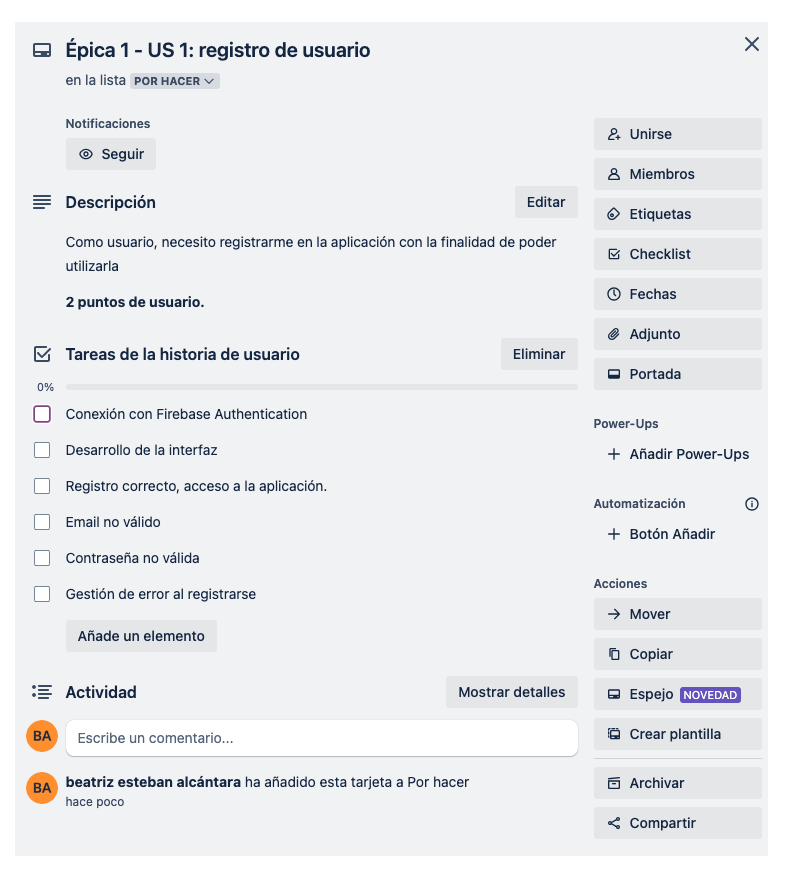
\includegraphics[width=0.6\textwidth]{./img/requirements/user_story_trello.png}
\caption{Historia de usuario en Trello}
\label{fig:user_story_trello}
\end{figure}

\begin{figure}[H]
\centering
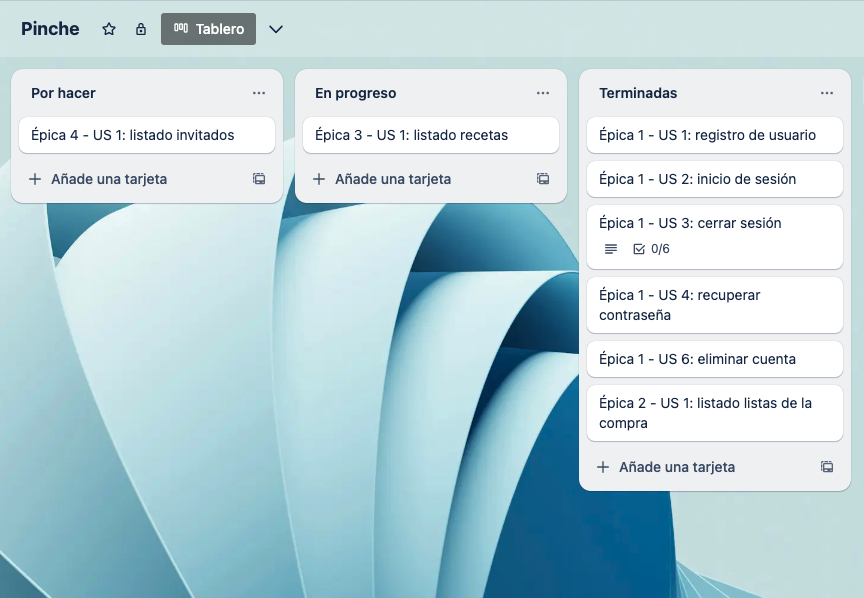
\includegraphics[width=0.6\textwidth]{./img/requirements/final_sprint_trello.png}
\caption{Estado del tablero Kanban al final del primer Sprint.}
\label{fig:final_sprint_trello}
\end{figure}

Tras la sesión de \textit{Sprint Review} y la de \textit{Sprint Retrospective}, se ajust\'o el alcance estimado para los siguientes Sprints a un m\'aximo de 8 puntos de historia por iteraci\'on, adaptando as\'i la velocidad al contexto real del desarrollo.

Una hoja resumen con todas las historias de usuario, agrupadas por \'epica, sus tareas y estimaciones, se adjunta en el anexo \texttt{Historias de usuario.xlsx}.

\subsection{Requisitos no funcionales}

Además de la funcionalidad, se han establecido los siguientes requisitos no funcionales:

\begin{itemize}
    \item \textbf{Aplicación nativa Android}, desarrollada con \textbf{Kotlin} y \textbf{Jetpack Compose}, para garantizar buen rendimiento y aprovechamiento de los recursos del dispositivo \cite{kotlin,jetpack}.
    \item \textbf{Persistencia de datos en la nube} mediante \textbf{Firebase Firestore} para facilitar el acceso a la información desde diferentes dispositivos \cite{firestore}.
    \item \textbf{Autenticación de usuarios} mediante \textbf{Firebase Authentication}, garantizando un sistema de acceso seguro y sencillo \cite{firebase-auth}.
    \item \textbf{Interfaz centrada en la experiencia de usuario}, basada en los principios de diseño de Google Material Design.
    \item \textbf{Estructura modular y escalable}, basada en el patrón arquitectónico \textbf{MVVM} (Model-View-ViewModel).
\end{itemize}

Estos requisitos definen el alcance funcional y técnico del proyecto, garantizando que el producto final responda tanto a las expectativas del usuario como a criterios de calidad del software.


\section{Arquitectura y análisis}
\label{sec:arquitectura-analisis}

La arquitectura de una aplicación móvil resulta crítica para garantizar su escalabilidad, optimización del código, rendimiento, solidez, mantenibilidad,y la correcta separación de responsabilidades. En este proyecto se ha adoptado la arquitectura recomendada por Android, basada en una estructura en capas y el patrón MVVM (Model-View-ViewModel), con la inclusión de una capa de dominio opcional y la gestión de dependencias mediante Hilt.

\subsection{Principios generales}

Esta arquitectura promueve los principios de separación de responsabilidades, flujo unidireccional de datos, modularidad y testabilidad \cite{android-architecture}. El modelo propuesto divide la lógica de la aplicación en tres capas principales: UI, dominio (opcional) y datos, Figura~\ref{fig:mvvm}. En nuestro caso vamos a utilizar la arquitectura recomendada incluyendo la capa opcional de dominio.

\begin{figure}[H]
\centering
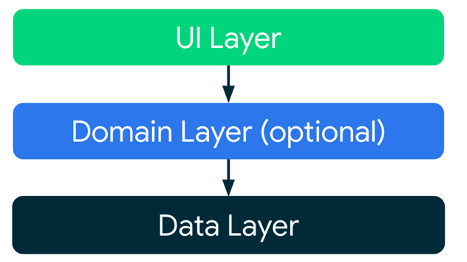
\includegraphics[width=0.6\textwidth]{./img/mvvm.png}
\caption{Diagrama arquitectura MVVM.}
\label{fig:mvvm}
\vspace{0.2em}
{\footnotesize \centering \textit{Fuente:} \url{https://developer.android.com/topic/architecture?hl=es-419} \par}
\end{figure}

\subsection{Capa de UI}

La capa de interfaz de usuario es responsable de mostrar los datos al usuario y recoger sus interacciones. Esta capa se compone de dos tipos de elementos:

\begin{itemize}
    \item \textbf{Elementos de la UI}: Son funciones de Jetpack Compose que renderizan los datos en pantalla.
    \item \textbf{Contenedores de estado}: Los ViewModel que retienen el estado de la UI y exponen datos reactivos mediante \texttt{StateFlow}.
\end{itemize}

\subsection{Capa de dominio}

La capa de dominio encapsula la lógica empresarial que puede ser compartida entre distintos ViewModels. En ella se definen los casos de uso (\textit{use cases}) como clases que representan acciones o procesos específicos de la aplicación, facilitando la reutilización de código y la claridad del flujo de datos.

\subsection{Capa de datos}

Esta capa es responsable de la obtención y persistencia de datos, ya sea desde fuentes remotas como Firebase Firestore, o locales. Se organiza en:

\begin{itemize}
    \item \textbf{Repositorios}: Actúan como intermediarios entre las fuentes de datos y la capa de dominio.
    \item \textbf{Fuentes de datos}: Pueden ser locales o remotas. En nuestro caso, son remotas: usamos Firebase que proporciona servicios de autenticación y base de datos en la nube \cite{firestore, firebase-auth}.
\end{itemize}

Gracias a esta separación, si en el futuro se quisiera cambiar de base de datos (por ejemplo, de Firebase a Amazon DynamoDB), solo se vería afectada la capa de datos, manteniendo intacto el resto del sistema.

\subsection{Gestión de dependencias con Hilt}

La gestión de dependencias se realiza mediante la biblioteca Hilt, un contenedor de inyección de dependencias desarrollado por Google. Hilt proporciona objetos preconfigurados a las clases de Android y administra automáticamente su ciclo de vida \cite{hilt-android}. Esto permite:

\begin{itemize}
    \item Reducir el acoplamiento entre componentes.
    \item Facilitar el testeo gracias a la posibilidad de sustituir dependencias reales por versiones simuladas.
    \item Garantizar la escalabilidad del código mediante una configuración declarativa y reutilizable.
\end{itemize}

\subsection{Ventajas de esta arquitectura}

La aplicación Pinche se beneficia de esta arquitectura al conseguir:

\begin{itemize}
    \item Mejor separación de responsabilidades entre componentes.
    \item Mayor facilidad de testeo en todas las capas.
    \item Reutilización de lógica empresarial entre distintas pantallas.
    \item Facilidad para mantener y escalar el código base en el futuro.
\end{itemize}

Este enfoque permite un desarrollo estructurado, coherente y sostenible, favoreciendo además la implementación de buenas prácticas de ingeniería de software.


\section{Diseño e implementación}
\label{sec:diseno-implementacion}

El desarrollo de la aplicación \textbf{Pinche} se ha centrado en aplicar buenas prácticas de ingeniería de software para Android, incluyendo el patrón MVVM, el uso de Jetpack Compose y la organización modular del código.

\subsection{Análisis de requerimientos y estructura funcional}

La aplicación ha sido diseñada en base a un conjunto de funcionalidades organizadas en tres secciones principales: listas de la compra, recetas e invitados. Este enfoque permite abordar de forma modular las necesidades de los usuarios y facilita la extensión del sistema.

El modelo de datos se ha estructurado para cubrir las siguientes entidades principales:

\begin{itemize}
    \item \textbf{Lista}: contiene un conjunto de productos, su nombre y estado.
    \item \textbf{Producto}: asociado a una lista, con nombre, cantidad y supermercado.
    \item \textbf{Receta}: incluye nombre, pasos de elaboraci\'on, ingredientes y número de comensales.
    \item \textbf{Ingrediente}: definido por nombre y cantidad relativa a los comensales.
    \item \textbf{Invitado}: con nombre, preferencias alimentarias, intolerancias y registro de comidas anteriores.
\end{itemize}

Este modelo facilita la integración de funcionalidades como el cálculo de ingredientes según el número de comensales, la generación de listas automáticas a partir de recetas y la personalización de menús para invitados con restricciones.

\subsection{Patr\'on MVVM}

El patrón Model-View-ViewModel (MVVM) permite una clara separación de responsabilidades entre la interfaz de usuario y la lógica de negocio. Esta estructura permite un mejor testeo, una mayor mantenibilidad del código y una arquitectura reactiva orientada al ciclo de vida del sistema \cite{viewmodel}.

\begin{itemize}
    \item \textbf{Model}: representa la capa de datos de la aplicación, incluyendo los repositorios y el acceso a Firestore.
    \item \textbf{View}: implementada usando Jetpack Compose, se encarga de mostrar los datos y de capturar la interacción del usuario.
    \item \textbf{ViewModel}: contiene la lógica de presentación, retiene el estado y orquesta el flujo de datos entre View y Model usando \texttt{StateFlow}.
\end{itemize}

\subsection{Jetpack Compose y su integraci\'on}

Jetpack Compose es el framework de UI moderno de Android, que permite declarar interfaces de forma reactiva con funciones de Kotlin \cite{jetpack}. Gracias a su enfoque declarativo, se reduce la cantidad de código boilerplate y se mejora la legibilidad del código fuente.

Ejemplo de composable en la aplicación:

\begin{verbatim}
@Composable
fun RecipeCard(recipe: Recipe) {
    Card(modifier = Modifier.padding(8.dp)) {
        Column {
            Text(text = recipe.name, style = MaterialTheme.typography.h6)
            Text(text = "Comensales: ${recipe.servings}")
        }
    }
}
\end{verbatim}

\subsection{Decisiones técnicas relevantes}

Durante el desarrollo se tomaron decisiones clave como:

\begin{itemize}
    \item Uso de \textbf{Jetpack Navigation} para gestionar la navegación entre pantallas de manera estructurada.
    \item Implementación de \textbf{Hilt} para inyección de dependencias, facilitando el testeo y la escalabilidad.
    \item Empleo de \textbf{StateFlow} para la gestión del estado de la UI, evitando fugas de memoria.
    \item Utilización de \textbf{Git} como sistema de control de versiones, junto con ramas por tarea y buenas prácticas de integración continua (CI).
    \item Desarrollo colaborativo organizado a través de tableros \textbf{Trello} y prototipos creados en \textbf{Figma}.
\end{itemize}

Esta implementación modular y centrada en buenas prácticas garantiza que Pinche pueda mantenerse y escalarse en el tiempo, facilitando la extensi\'on de funcionalidades futuras.

\section{Pruebas}
\label{sec:pruebas}

El aseguramiento de la calidad en el desarrollo de la aplicación \textbf{Pinche} se ha abordado mediante una estrategia de pruebas estructurada que cubre distintos niveles de validación del sistema: pruebas unitarias, de interfaz, de integración, de extremo a extremo (E2E) y cobertura de código. Esta estrategia ha permitido verificar que los componentes funcionan correctamente de forma individual y en conjunto.

\subsection{Pruebas unitarias}

Las pruebas unitarias validan pequeñas unidades de código de forma aislada, principalmente funciones puras o clases sin dependencias externas. Para ello se ha utilizado \textbf{JUnit4} como framework base, complementado con \textbf{MockK} para simular comportamientos de dependencias externas como repositorios o servicios \cite{android-testing}.

MockK se ha elegido frente a otras alternativas como Mockito debido a su compatibilidad nativa con Kotlin, su soporte para coroutines y su sintaxis más idiomática.

el Listado~\ref{lst:signinTest},

\begin{lstlisting}[language=Java, caption={SignInUserUseCaseTest}, label={lst:signinTest}]
  @ExperimentalCoroutinesApi
  class SignInUserUseCaseTest {

    @get:Rule
    val coroutinesTestRule = MainDispatcherRule()

    private val authRepository: AuthRepository = mockk()
    private lateinit var signInUserUseCase: SignInUserUseCase

    private val email = "test@example.com"
    private val password = "123456"

    @Before
    fun setup() {
        signInUserUseCase = SignInUserUseCase(authRepository)
    }

    @Test
    fun `sign in returns Success when repository succeeds`() = runTest {
        coEvery { authRepository.firebaseSignInWithEmailAndPassword(email, password) } returns Success(true)

        val result = signInUserUseCase(email, password)

        assertTrue(result is Success)
        coVerify { authRepository.firebaseSignInWithEmailAndPassword(email, password) }
    }

    @Test
    fun `sign in returns Failure when repository fails`() = runTest {
        val exception = Exception("Auth error")
        coEvery { authRepository.firebaseSignInWithEmailAndPassword(email, password) } returns Failure(exception)

        val result = signInUserUseCase(email, password)

        assertTrue(result is Failure)
        coVerify { authRepository.firebaseSignInWithEmailAndPassword(email, password) }
    }
}
\end{lstlisting}

\subsection{Pruebas de interfaz (UI)}

Para comprobar el comportamiento de la interfaz de usuario, se ha utilizado la librería \texttt{androidx.compose.ui:ui-test-junit4}, integrada en Jetpack Compose. Esta herramienta permite verificar la presencia de elementos, sus estados, y simular acciones del usuario como clics o introducción de texto.

Frente a otras librerías tradicionales como Espresso, esta herramienta ofrece mejor sincronización con el ciclo de recomposición de Compose y facilita pruebas más declarativas \cite{android-testing}.

\subsection{Pruebas de integración}

Las pruebas de integración validan que múltiples componentes trabajen juntos de forma coherente. En este proyecto se han utilizado:

\begin{itemize}
    \item \textbf{Firebase Emulator Suite}, que simula los servicios de Firebase (Firestore y Auth) localmente \cite{firebase-emulator}.
    \item \textbf{Repositorios simulados} combinados con \textbf{Hilt} para sustituir dependencias reales durante las pruebas.
\end{itemize}

Este enfoque permite realizar pruebas realistas pero controladas, sin depender de servicios externos ni afectar datos en producción.

\subsection{Pruebas end-to-end (E2E)}

Las pruebas E2E verifican que la aplicación funciona correctamente en su conjunto, desde la interacción del usuario hasta el acceso a datos y navegación.

Se ha empleado \textbf{Espresso}, el framework oficial de Google para pruebas E2E en Android, junto con Firebase Emulator Suite para simular los servicios remotos. Estas pruebas son útiles para validar flujos completos como el inicio de sesión, la creación de listas o la adición de productos \cite{android-testing}.

\subsection{Cobertura de código}

Como métrica adicional de calidad, se ha utilizado \textbf{JaCoCo} para generar informes de cobertura de código. Esto permite conocer qué líneas del proyecto han sido ejecutadas durante las pruebas y detectar zonas sin cobertura suficiente \cite{jacoco}.

JaCoCo se integra fácilmente con Gradle y Android Studio, proporcionando estadísticas precisas que se han utilizado para ajustar el alcance de las pruebas implementadas.
